%%%%%%%%%%%%%%%%%%%%%%%%%%%%%%%%%%%%%%%%%%%%%%%%%%%%%%%%%%%%%%%%%%%%%%%%%%%%%%%%
%2345678901234567890123456789012345678901234567890123456789012345678901234567890
%        1         2         3         4         5         6         7         8

\documentclass[letterpaper, 12 pt, conference]{ieeeconf}  % Comment this line out
                                                          % if you need a4paper
%\documentclass[a4paper, 10pt, conference]{ieeeconf}      % Use this line for a4
                                                          % paper

\IEEEoverridecommandlockouts                              % This command is only
                                                          % needed if you want to
                                                          % use the \thanks command
\overrideIEEEmargins
% See the \addtolength command later in the file to balance the column lengths
% on the last page of the document


\usepackage{fullpage}
\usepackage{graphicx}

% The following packages can be found on http:\\www.ctan.org
\usepackage{graphicx} % for pdf, bitmapped graphics files
\usepackage{bm}
\newcommand{\uvec}[1]{\boldsymbol{\hat{\textbf{#1}}}}
%\usepackage{epsfig} % for postscript graphics files
%\usepackage{mathptmx} % assumes new font selection scheme installed
%\usepackage{times} % assumes new font selection scheme installed
%\usepackage{amsmath} % assumes amsmath package installed
%\usepackage{amssymb}  % assumes amsmath package installed

\title{\LARGE \bf
Using Artificial Neural Networks for Instrument Classification of Audio Signals
}


\author{Saksham Goel% <-this % stops a space
%\thanks{}% <-this % stops a space
%\thanks{$^{1}$Saksham Goel, Student - Department of Computer Science, University of Minnesota - Twin Cities}%
}


\begin{document}



\maketitle
\thispagestyle{empty}
\pagestyle{empty}


%%%%%%%%%%%%%%%%%%%%%%%%%%%%%%%%%%%%%%%%%%%%%%%%%%%%%%%%%%%%%%%%%%%%%%%%%%%%%%%%
\begin{abstract}
This project examines the applications of using different types of Deep Learning Architectures like Recurrent Neural Networks (RNN) and Convolutional Neural Networks (CNN) for instrument recognition. The project is divided into two section. First section of the project explores the time dependency of the audio signals hence uses architectures like Simple Vanilla RNN, Gated Recurrent Unit (GRU) \cite{gru_translation}, Long Short Term Memory (LSTM) \cite{lstm_sequence_modelling} \cite{lstm_music_genre} and Bidirectional Long Short Term Memory (BLSTM) \cite{bidirectional_lstm_speech}. Second section on the contrary explores the local dependency of the audio signals hence uses techinuqes like CNN's on top of Multiresolution Recurrence Plots (MRP) \cite{cnn_music_mrp} and RNN's on top of CNN's \cite{cnn_rnn_sleep_staging}.
\end{abstract}


%%%%%%%%%%%%%%%%%%%%%%%%%%%%%%%%%%%%%%%%%%%%%%%%%%%%%%%%%%%%%%%%%%%%%%%%%%%%%%%%
%                                   INTRODUCTION                               %
% Topics Covered
%   1. Problem Statement
%   2. Algorithm Used (Recurrent Neural Network Architectures)
%%%%%%%%%%%%%%%%%%%%%%%%%%%%%%%%%%%%%%%%%%%%%%%%%%%%%%%%%%%%%%%%%%%%%%%%%%%%%%%%
\section{INTRODUCTION}

Music is one of the most popular source of entertainment for us humans and boasts one of the biggest entertainment industries. A lot of research is being done currently for novel ways of queriying music and sound signals. This project aims to set up a proof of concept for using different deep learning architectures for the task of instrument classification of audio signals so that it can be used to label sound recordings. This project focuses pn training different deep learning architectures as mentioned in the abstract and performing a comparison of the accuracies. The problem statement is as follows: \textit{Given an audio signal with a predoiminated sound of a given instrument, the model will classify some $t$ second sliding windows of that given audio excerpt into one category from any of the following categorie mentioned in Table \ref{tab:pd}.}

Audio recognition is very widely researched filed in todays time. A lot of research is being conducted in the field of speech recognition to make the existing phone assitants like Siri, Google Home better and much more accurate. Audio data is very special because of its inherent structure which dictates dependency between sound signals at two different signals. To think about it, audio signals are temporal data much like time series data such that they have long range dependency between signals. Because of this property it is hard to use traditional machine learning algorithms because they make assumptions like the features of the data are independent and identically distributed. One of the most popular deep learning architecture used in the field of dependent values and modeling time series like data is Recurrent Neural Networks. They have been proven effective in sequence modelling \cite{gru_evaluation} and also in handling temporal data of varying lengths \cite{gru_evaluation}. RNN stores the information about time series in a hidden unit and use these to actually compute the output values which is why they are excellent at modelling Time-Series data. For this project we are using the following $4$ types of RNN's:

\begin{description}
	\item [$\bullet$ Simple Vanilla RNN (Figure: \ref{fig:RNN})]
	\item [$\bullet$ Long Short Term Memory (Figure: \ref{fig:LSTM})]
	\item [$\bullet$ Gated Recurrent Unit (Figure: \ref{fig:GRU})]
	\item [$\bullet$ Bidirectional Long Short Term Memory]
\end{description}

Other than modelling the audio signals using architectures focusing on time series data, I will also try to use Convolutional Neural Network for modelling neighboring value dependencies. This project with use the following $3$ types of CNN's:
\begin{description}
	\item [$\bullet$ Simple Vanilla CNN (Figure: \ref{fig:CNN})]
	\item [$\bullet$ CNNs on MRP]
	\item [$\bullet$ CNN + RNN] 
\end{description}

%One of them is called Gated Recursive Neural Network which features a block named Gated Recurrent Unit (GRU) which is extensivley used in fields of machine translation \cite{cho2014properties}. The other architecture is called Long Short-Term Memory Recurrent Neural Network which features a block named LSTM unit \cite{graves2013generating}. The advantage of using LSTM architecture is that LSTM is very good at solving the problem of vanishing gradients when the data has very long temporal dependencies. With the inclusion of different gates (inherent computations to calculate the hidden state) like memory and forget gates which affect the computation of the hidden state, LSTM essentially can use the values to include the memory from previous timesteps and influence the output accordingly, hence effectively capturing long distance temporal dependencies. On the other hand GRU is very much similar to LSTM using different gates, but has a different architecture for the GRU unit. GRU combines some of the gates in LSTM cell (like forget and input gate) to essentially reduce the number of learnable parameters. Due to this, both of them differ in the way they let the output affect the memory inclusion, and also how the output value is calculated \cite{chung2014empirical}, while trying to solve the same problem of long term temporal dependencies. The advantage of GRU over LSTM is that it used smaller set of learnable parameters and hence is easier to train and expected to reach a state of convergence much faster. On the other hand advantages of LSTM is that they can learn more abstract long term dependencies because of their intricate structure. Considering that the audio data has a high number of features (a lot of sound signals in the 3 second window \textbackslash 1.2 Million sound signals per 3 second window) it will be good to use GRU so that we can essentially train the model easily and reach convegence early, however LSTM may proove to be more accurate.

%RNNs are composed of small unit called RNN Cells, the main idea behind Recurrent Neural Networks is to store a hidden state (a feature vector) that represents the current state of the RNN cell. This hidden state is computed using the input values and the hidden state value from the previous cell. Hence, whenever we initialize a RNN it is important to initialize the hiddent state for the first cell ($h_0$) and the matrices used for the computation. This kind of architecture resembles a dependency of the current hidden state value on the previous hidden state values and the current input value. In mathematical terms we can see that the equation looks somthing like:
%\begin{center}
%$h_t = f(x_t, h_{t-1})$
%\end{center}

%In this project we are concerned with analyzing audio signals. Because audio signals are inherently like time series, such that the value of audio signals are time dependent, we focused on using Recurrent Neural Network as one of the main architectures. RNN's were the top choice because they take into considertion the time dependency of the signals (values) and use a hidden state to do computations and store information. For the first section of the project apart from Simple Vanilla RNN, I am using LSTM because of their ability for modelling long term dependencies and being able to 


%%%%%%%%%%%%%%%%%%%%%%%%%%%%%%%%%%%%%%%%%%%%%%%%%%%%%%%%%%%%%%%%%%%%%%%%%%%%%%%%
%                                   RESOURCES                                  %
% Topics Covered
%   1. What technology will be used?
%   2. Python Libraries and amount of code that can be reused
%%%%%%%%%%%%%%%%%%%%%%%%%%%%%%%%%%%%%%%%%%%%%%%%%%%%%%%%%%%%%%%%%%%%%%%%%%%%%%%%
\section{RESOURCES}

\subsection{Dataset}
The techinuqes we are using for this project are supervised learning algorithms hence we require data with annotations about the class they belong to. For this project we are using the Instrument Recognition in Music Audio Signals (IRMAS) Dataset \cite{IRMAS_Dataset}. The IRMAS dataset currently has divided the dataset into Training and Test sets. Training dataset contains 6705 audio excerpts in 16 bit stereo wav format audio files sampled at 44.1 kHz. All of these files are 3 second excerpts from more than 2000 distinct recordings. The number of audio files for a subset of all classes that I will be training on is given in Table \ref{tab:pd}. For the test set there are 2874 excerpts in 16 bit stereo wav format sampled at 44.1kHz.

\begin{table}
\centering
\caption{Number of Training Samples by Instrument Class}
\begin{tabular}{| c || c |} %sets the format of the table
\hline %horizontal line
 Instrument Category &  Number of Audio Files \\
   \hline \hline
\hline
Electric Guitar &  760 \\
\hline
Piano  &   721 \\
\hline
Saxophone  &   626 \\
\hline
Violin &   580 \\
\hline
Human Singing Voice  &   778 \\
\hline
   \end{tabular}
\label{tab:pd} 
\end{table}


\subsection{Implementation}
For this project the implementation will all be done in Python. Python is an open source interpreted high-level programming language for general-purpose programming. Currently python supports a lot of powerful libraries like Keras, Tensorflow and Pytorch which provide enough resources to set up different deep learning architectures that have been mentioned before. Along with these libraries there also exist some other libaries like numpy, scipy, sklearn and matplotloib which will help in data loading, preprocessing, analysis and visualizations. All of these libaries have lots of great documentation available online and also a lot of blog articles on websites like Medium and TowardsDataScience containing helpful resources related to the full spectrum. On my initial analysis, there is not much code available online directly corresponding to my problem. I will be coding the chunk of the whole project but most of it will be based off online discussions and blogs where people try to use these architectures for different yet similar problems.

%%%%%%%%%%%%%%%%%%%%%%%%%%%%%%%%%%%%%%%%%%%%%%%%%%%%%%%%%%%%%%%%%%%%%%%%%%%%%%%%
%                                   EXPERIMENT                                 %
% Topics Covered
%   1. Data 
%   2. Different experiments that I will run?
%   3. Assumptions
%%%%%%%%%%%%%%%%%%%%%%%%%%%%%%%%%%%%%%%%%%%%%%%%%%%%%%%%%%%%%%%%%%%%%%%%%%%%%%%%
\section{EXPERIMENT}

For this project I will be setting up different experiments in different notebooks that will walkthrough what type of experiment is being conducted along with the final assessment of that experiment. Most of the experiments would correspond to using different architectures with the same input dataset and similar values of the hyperparameters. For this part of the experiment, I would first compare all the 4 types of RNN's for some binary classification and then compare them on the multiclass comparison containing all the classes that I am considering. Similarly I would also experiment with the two types of CNN models discussed earlier with binary and multiclass classification. These experiments would lead to analysis based on using different architectures for the same dataset over the type of classification being performed. The other type of experiments that I will be performing includes experimenting with the data preprocessing which includes different types of normalization (mean normalization, variance normalization, uniform normalization) on the data and also experimenting with windowing techniques which would deal with the amount of data being loaded. I am especially considered with windowing because it would highly affect the amount of data on which I will be training and also the values of the audio signal I will be using. I am planning to experiment with different sliding window sizes to get a better understanding of the effect of the initial dataset size on the classification accuracy of the model. Other than these I will also do some experimentation to understand the effect of hyperparameters of the architectures on their performance. These experiments however would be each architecture specific. For hyperparameters I will be experimenting with different activation functions, dropout percentages, number and size of layers.


%%%%%%%%%%%%%%%%%%%%%%%%%%%%%%%%%%%%%%%%%%%%%%%%%%%%%%%%%%%%%%%%%%%%%%%%%%%%%%%%
%                                   TIMELINE                                   %
% Topics Covered
%   1. SCHEDULE
%%%%%%%%%%%%%%%%%%%%%%%%%%%%%%%%%%%%%%%%%%%%%%%%%%%%%%%%%%%%%%%%%%%%%%%%%%%%%%%%
\section{TIMELINE}

This project has a lot of different parts belonging to it. Hence for the timeline I have divided it into many parts, such that each deal with a particular part of the whole project and the pipeline that needs to be created. The different parts of the pipeline is as follows:

\begin{enumerate}
  \item Dataset exploration, exploring different online available datasets. 
  \item Data loader, developing scripts for loading data from the sample audio files. This includes loading data in the format usable by RNN and loading data usable by CNN.
  \item Data preprocessing, developing scripts to preprocess the data. This includes normalizing, sliding windows and also constructing MRP.
  \item Model training, developing Ipython notebooks that will load data from the given training data and fit different models with a particular set of hyperparameters on the training data.
  \item Visualization, developing Ipython notebooks to visualize the convergence, loss and accuracy plots.
  \item Analyzing results, developing Ipython notebooks that will run inference on test data and calculate different accuracy metrics like precision, recall, overall classification accuracy, F-1 score.
  \item Hyperparameter Tuning, doing some experimentation with different hyperparameters for the model architectures and retraining and redoing the analysis.
  \item Conclusion, discussing the different results and trying to understand why id we get such results.
\end{enumerate}



%%%%%%%%%%%%%%%%%%%%%%%%%%%%%%%%%%%%%%%%%%%%%%%%%%%%%%%%%%%%%%%%%%%%%%%%%%%%%%%%
%                                   ANALYSIS                                   %
% Topics Covered
%   1. What will be analyzed
%   2. How will I analyze it?
%%%%%%%%%%%%%%%%%%%%%%%%%%%%%%%%%%%%%%%%%%%%%%%%%%%%%%%%%%%%%%%%%%%%%%%%%%%%%%%%
\section{ANALYSIS}

For this project I will be analyzing the classification accuraccy of the models on a seperate hold out test set after they have been trained. For the evaluation purposes I will be using three different metrics which are classification accuracy, precision and recall. For terms of analysis, I will draw some confusion matrices for comparsion of the overall accuraccies, precision and recall while also use the confusionmatrix to create a heatmap for easy visualization. I will also consider the amount of iterations it took for different models to converge and overall complexity of the models. Considering all these facts together I will try to analyze why each model performs the way it performs and try to select a model which seems to maximize the accuraccy while minimizing the complexity and convergence time. Because I will be performing a lot of experiments and each experiments tries to change one particular variable like model architecture or hyperparameters or data preprocessing, it will help me create a lot of different tables where I will discuss the affect of each variable as well which will help in learning about the effect of each variable when thinking about them in domain of Audio Classification. 

\section{APPENDIX: A}

Images for different architectures that have been referred in this writeup.

\begin{figure*}[!h]
\centering
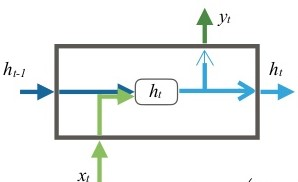
\includegraphics[scale=0.8]{../figs/rnn.jpg}	
\caption{RNN cell}
\label{fig:RNN} 
\end{figure*}

\begin{figure*}[!h]
\centering
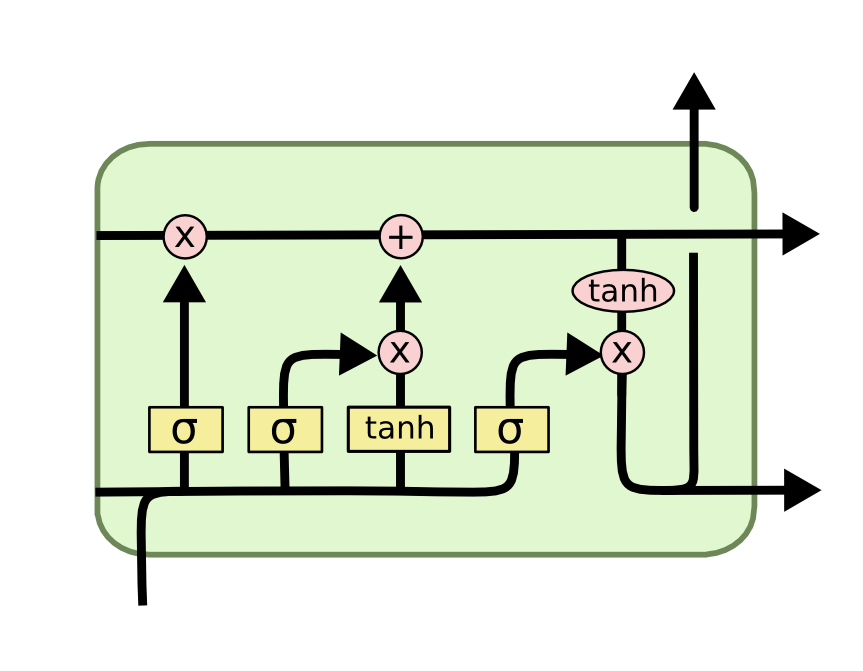
\includegraphics[scale=0.5]{../figs/lstm.png}	
\caption{LSTM cell}
\label{fig:LSTM} 
\end{figure*}

\begin{figure*}[!h]
\centering
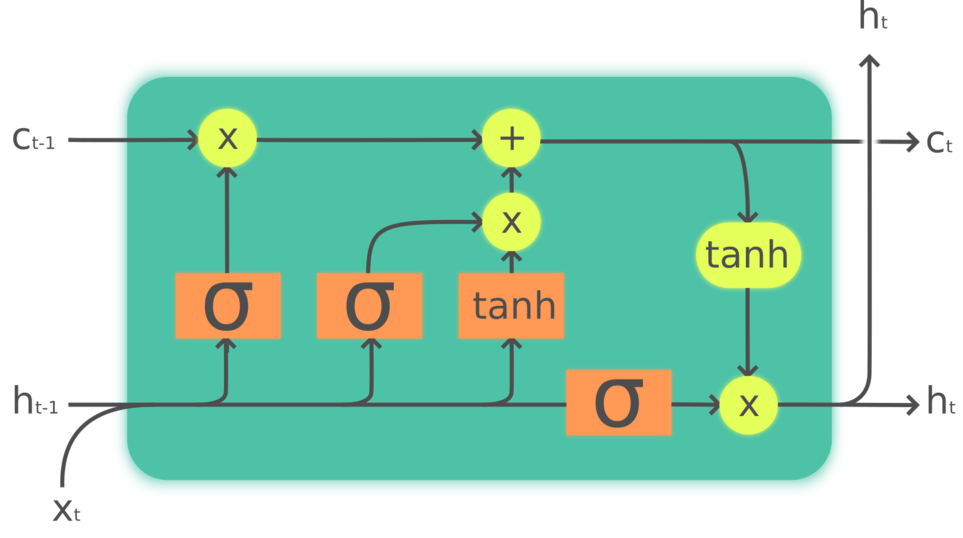
\includegraphics[scale=0.8]{../figs/gru.png}	
\caption{GRU cell}
\label{fig:GRU} 
\end{figure*}


\begin{figure*}[!h]
\centering
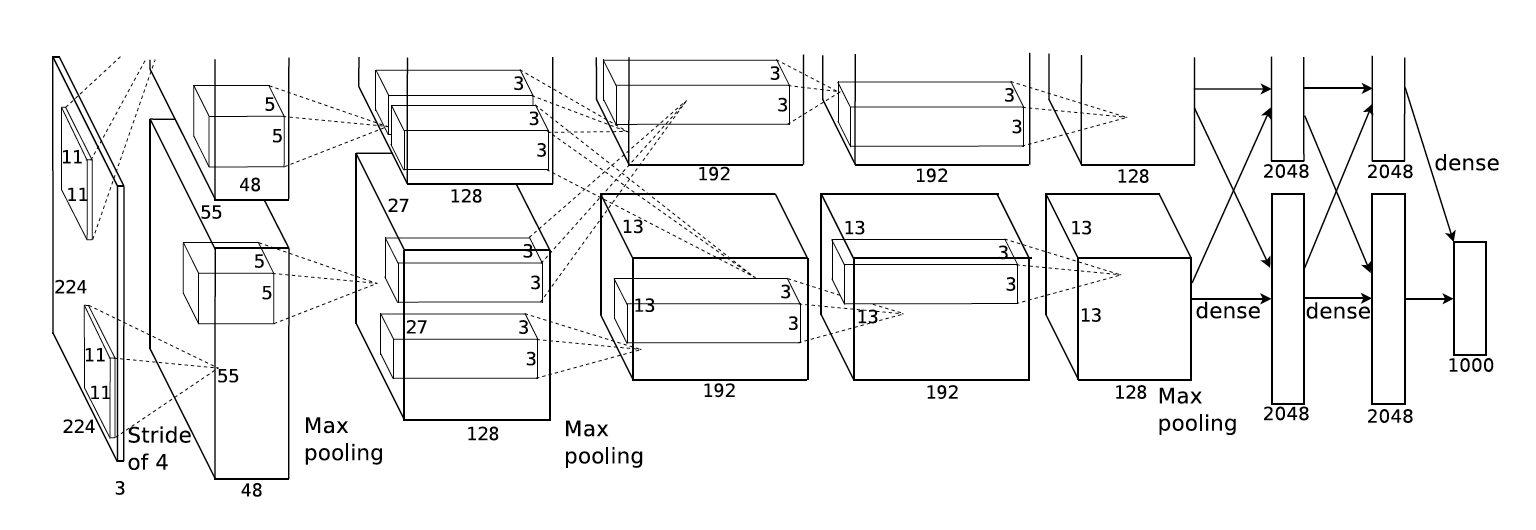
\includegraphics[width=\textwidth,height=5cm]{../figs/cnn.png}	
\caption{CNN architecture (Alexnet)}
\label{fig:CNN} 
\end{figure*}


\begin{thebibliography}{99}

\bibitem{IRMAS_Dataset} Bosch, Juan J., et al. "A Comparison of Sound Segregation Techniques for Predominant Instrument Recognition in Musical Audio Signals." ISMIR. 2012.

\bibitem{google_accoustics} Sak, Haşim, Andrew Senior, and Françoise Beaufays. "Long short-term memory recurrent neural network architectures for large scale acoustic modeling." Fifteenth annual conference of the international speech communication association. 2014.

\bibitem{google_speech} Sak, Haşim, Andrew Senior, and Françoise Beaufays. "Long short-term memory based recurrent neural network architectures for large vocabulary speech recognition." arXiv preprint arXiv:1402.1128 (2014).

\bibitem{imagenet_original} Krizhevsky, Alex, Ilya Sutskever, and Geoffrey E. Hinton. "Imagenet classification with deep convolutional neural networks." Advances in neural information processing systems. 2012.

\bibitem{bidirectional_lstm_speech} Graves, Alex, and Navdeep Jaitly. "Towards end-to-end speech recognition with recurrent neural networks." International Conference on Machine Learning. 2014.

\bibitem{renet} Visin, Francesco, et al. "Renet: A recurrent neural network based alternative to convolutional networks." arXiv preprint arXiv:1505.00393 (2015).

\bibitem{gru_evaluation} Chung, Junyoung, et al. "Empirical evaluation of gated recurrent neural networks on sequence modeling." arXiv preprint arXiv:1412.3555 (2014).

\bibitem{gru_translation} Cho, Kyunghyun, et al. "On the properties of neural machine translation: Encoder-decoder approaches." arXiv preprint arXiv:1409.1259 (2014).

\bibitem{lstm_sequence_modelling} Graves, Alex. "Generating sequences with recurrent neural networks." arXiv preprint arXiv:1308.0850 (2013).

\bibitem{cnn_rnn_sleep_staging} Aggarwal, Karan, et al. "A Structured Learning Approach with Neural Conditional Random Fields for Sleep Staging."

\bibitem{cnn_music_mrp} Park, Taejin, and Taejin Lee. "Musical instrument sound classification with deep convolutional neural network using feature fusion approach." arXiv preprint arXiv:1512.07370 (2015).

\bibitem{lstm_music_genre} Tang, Chun Pui, et al. "Music Genre classification using a hierarchical Long Short Term Memory (LSTM) model." (2018).


\end{thebibliography}



\end{document}
